%% Based on a TeXnicCenter-Template by Gyorgy SZEIDL.
%%%%%%%%%%%%%%%%%%%%%%%%%%%%%%%%%%%%%%%%%%%%%%%%%%%%%%%%%%%%%

%------------------------------------------------------------
%
\documentclass{amsart}
%
%----------------------------------------------------------
% This is a sample document for the AMS LaTeX Article Class
% Class options
%        -- Point size:  8pt, 9pt, 10pt (default), 11pt, 12pt
%        -- Paper size:  letterpaper(default), a4paper
%        -- Orientation: portrait(default), landscape
%        -- Print size:  oneside, twoside(default)
%        -- Quality:     final(default), draft
%        -- Title page:  notitlepage, titlepage(default)
%        -- Start chapter on left:
%                        openright(default), openany
%        -- Columns:     onecolumn(default), twocolumn
%        -- Omit extra math features:
%                        nomath
%        -- AMSfonts:    noamsfonts
%        -- PSAMSFonts  (fewer AMSfonts sizes):
%                        psamsfonts
%        -- Equation numbering:
%                        leqno(default), reqno (equation numbers are on the right side)
%        -- Equation centering:
%                        centertags(default), tbtags
%        -- Displayed equations (centered is the default):
%                        fleqn (equations start at the same distance from the right side)
%        -- Electronic journal:
%                        e-only
%------------------------------------------------------------
% For instance the command
%          \documentclass[a4paper,12pt,reqno]{amsart}
% ensures that the paper size is a4, fonts are typeset at the size 12p
% and the equation numbers are on the right side
%
\usepackage{amsmath}%
\usepackage{amsfonts}%
\usepackage{amssymb}%
\usepackage{graphicx}

\usepackage[T1]{fontenc}
\usepackage{beton}
\usepackage{euler}
\usepackage{latexsym}
\usepackage{amsmath}
\usepackage{amssymb}
\usepackage{amsthm}


%------------------------------------------------------------
% Theorem like environments
%
\newtheorem{theorem}{Theorem}
\theoremstyle{plain}
\newtheorem{acknowledgement}{Acknowledgement}
\newtheorem{algorithm}{Algorithm}
\newtheorem{axiom}{Axiom}
\newtheorem{case}{Case}
\newtheorem{claim}{Claim}
\newtheorem{conclusion}{Conclusion}
\newtheorem{condition}{Condition}
\newtheorem{conjecture}{Conjecture}
\newtheorem{corollary}{Corollary}
\newtheorem{criterion}{Criterion}
\newtheorem{definition}{Definition}
\newtheorem{example}{Example}
\newtheorem{exercise}{Exercise}
\newtheorem{lemma}{Lemma}
\newtheorem{notation}{Notation}
\newtheorem{problem}{Problem}
\newtheorem{proposition}{Proposition}
\newtheorem{remark}{Remark}
\newtheorem{solution}{Solution}
\newtheorem{summary}{Summary}
\numberwithin{equation}{section}

\newcommand{\C}{{\mathbb  C}}
\newcommand{\R}{{\mathbb  R}}
\newcommand{\Z}{{\mathbb  Z}}
\newcommand{\N}{{\mathbb  N}}
\newcommand{\Q}{{\mathbb  Q}}

\makeatletter
\renewcommand{\leq}{\leqslant}
\renewcommand{\geq}{\geqslant}
\renewcommand{\Re}{{\operator@font Re\,}}
\renewcommand{\Im}{{\operator@font Im\,}}
\makeatother

\def\abs#1{\left|#1\right|} 
%--------------------------------------------------------
\begin{document}
\title[A Hydra in Fourier Space]{Taming a Hydra of Singularities in Fourier Space}
\author{Thomas Schmelzer}
\address[]
{Thomas Schmelzer \newline
\indent Winton Capital Management \newline
\indent Magdalen Centre, The Oxford Science Park, Oxford OX4 4GA, UK
}
\email[]{thomas.schmelzer@gmail.com}

%\author{Author Two}
%\curraddr[A.~Two]{Author Two current address, line 1\newline%
%\indent Author Two current address, line 2}%
%\email[A.~Two]{author-two@authortwo-inst.hu}%
%\urladdr{http://www.authortwo.uni-atwo.hu}
%
%\thanks{Thanks for Author One.}
%\thanks{Thanks for Author Two.}
%\thanks{This paper is in final form and no version of it will be submitted for
%publication elsewhere.}
\date{\today}
%\subjclass{Primary 05C38, 15A15; Secondary 05A15, 15A18} %
%\keywords{Keyword one, keyword two etc.}%
%\dedicatory{Dedicated to Giuliana Bordigoni}

%\begin{abstract}
%This is a sample document which shows the most important features of the AMS Journal
%Article class.
%\end{abstract}
\maketitle


\section{Introduction}
In \cite{BornemannSchmelzer} Bornemann and Schmelzer invited the reader to contemplate
a remarkable limit problem which involves an oscillatory integral of extreme nature.
Consider a function $f: \R \to \R$ that is integrable\footnote{A function $f: \R \to \R$ is integrable if $\int_{-\infty}^\infty f(x) dx$ exists. Bornemann and Schmelzer solved the problem for a larger class of functions. In their analysis is was sufficient for $f$ to be bounded and continuous. }. 
Does the sequence of violently oscillatory integrals
\begin{equation}\label{eq1}
I_n[f] = \frac{1}{\pi}\int_0^\pi f(\tan^{[n]}x)\,dx, \qquad n=1,2,3,\ldots,
\end{equation}
have a limit as $n$ approaches infinity? If so, what is the limit?
Here $\tan^{[n]}x = \tan \circ \tan \circ \cdots \circ \tan x$ denotes the n-fold iteration of the $\tan$ function. 

It is the dramatic behavior of $\tan^{[n]}x$ that inspired Bornemann to call this function the Hydra of singularities. The aggressive nature of this function is revealed already for small $n$. As $x$ moves from $0$ to $\pi$, the values of $\tan x$ go all the way from $0$ to $+\infty$ and then from $-\infty$ to $0$ after passing the singularity at $\pi/2$. The singularity at $\pi/2$ breeds infinitely many new singularities located at $x_k$ where $\tan x_k = (k+1/2) \pi$ with $k \in \Z$. Note that the values $x_k$ accumulate at $\pi/2$. 

This process repeats for each further iteration of $\tan$. Each singularity breeds countably many new singularities which accumulate in their respective ancestor. In Figure~1 we have tried to illustrate this rather wild behavior of the $\tan^{[n]}x$ iteration.

\begin{figure}[hb]
\begin{center}
\hspace*{-0.5mm}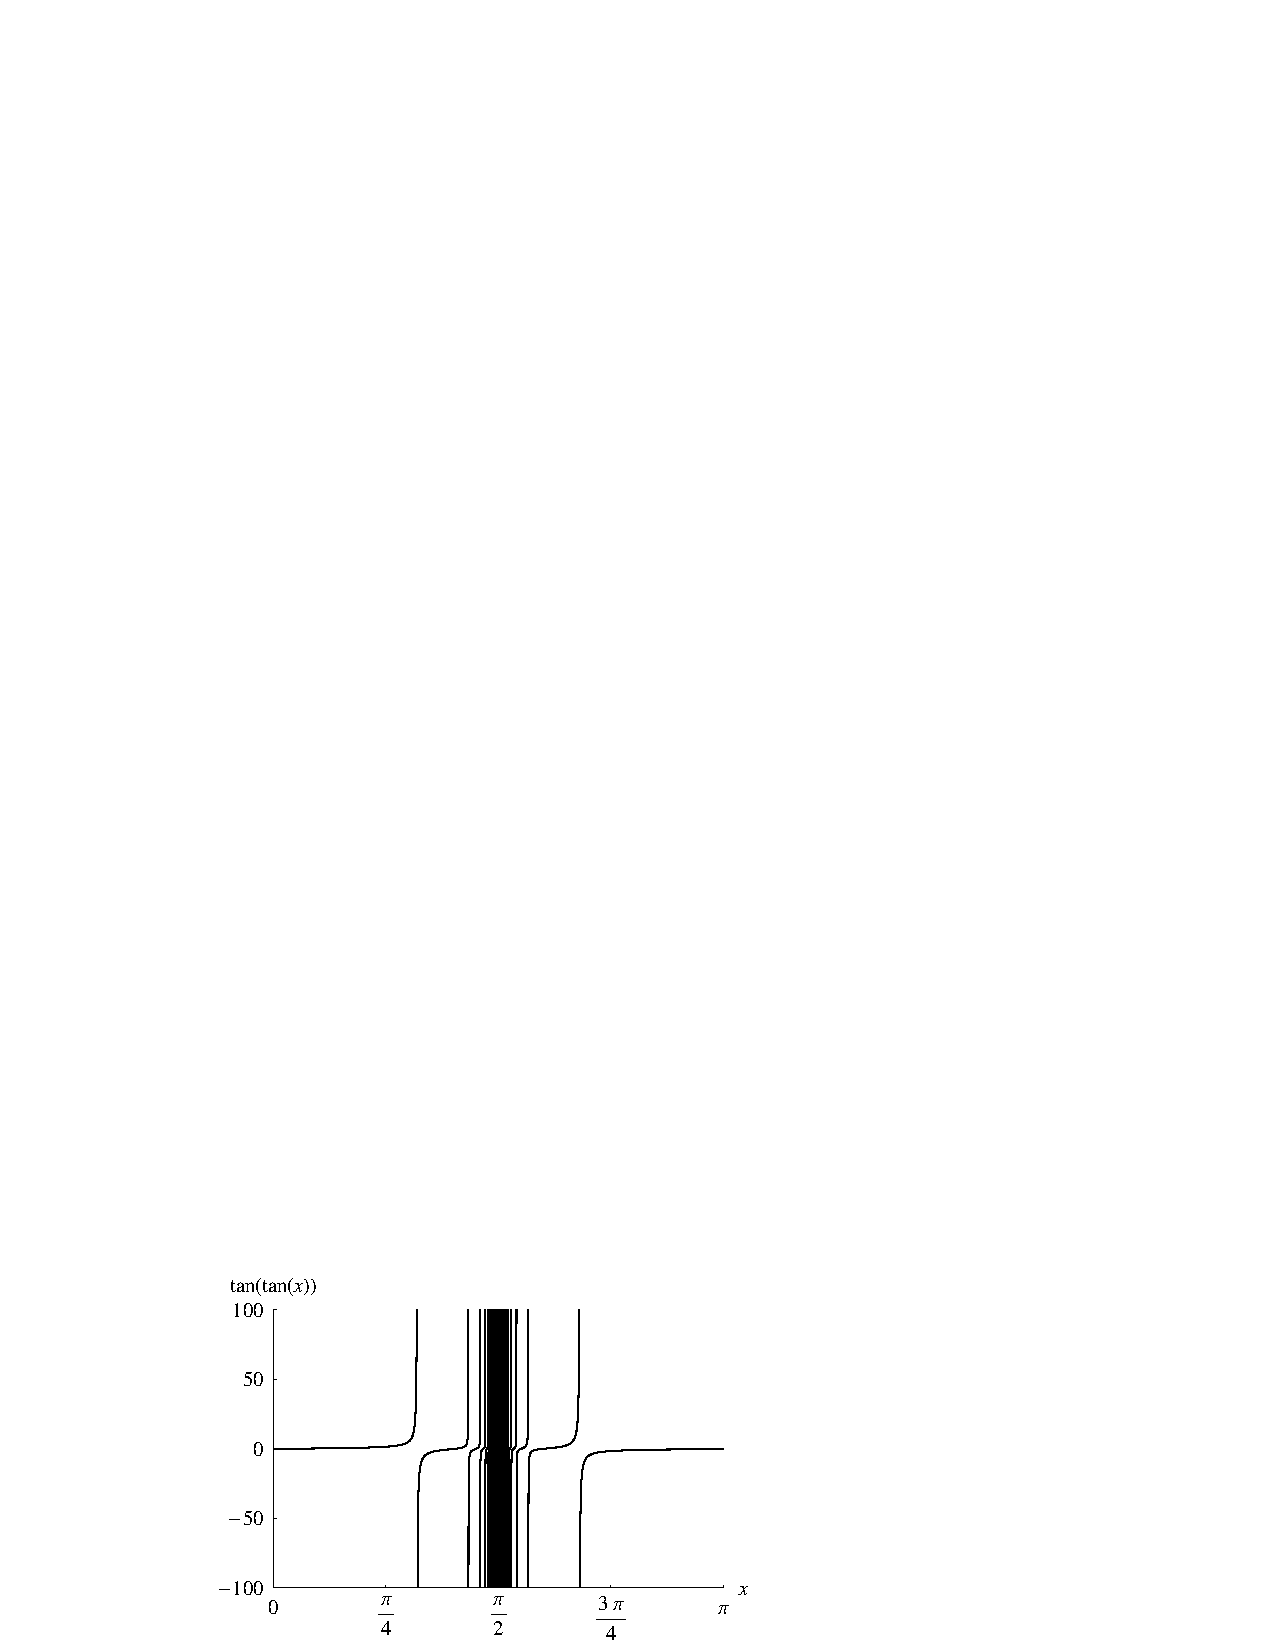
\includegraphics[scale=0.668]{tan2.pdf}\;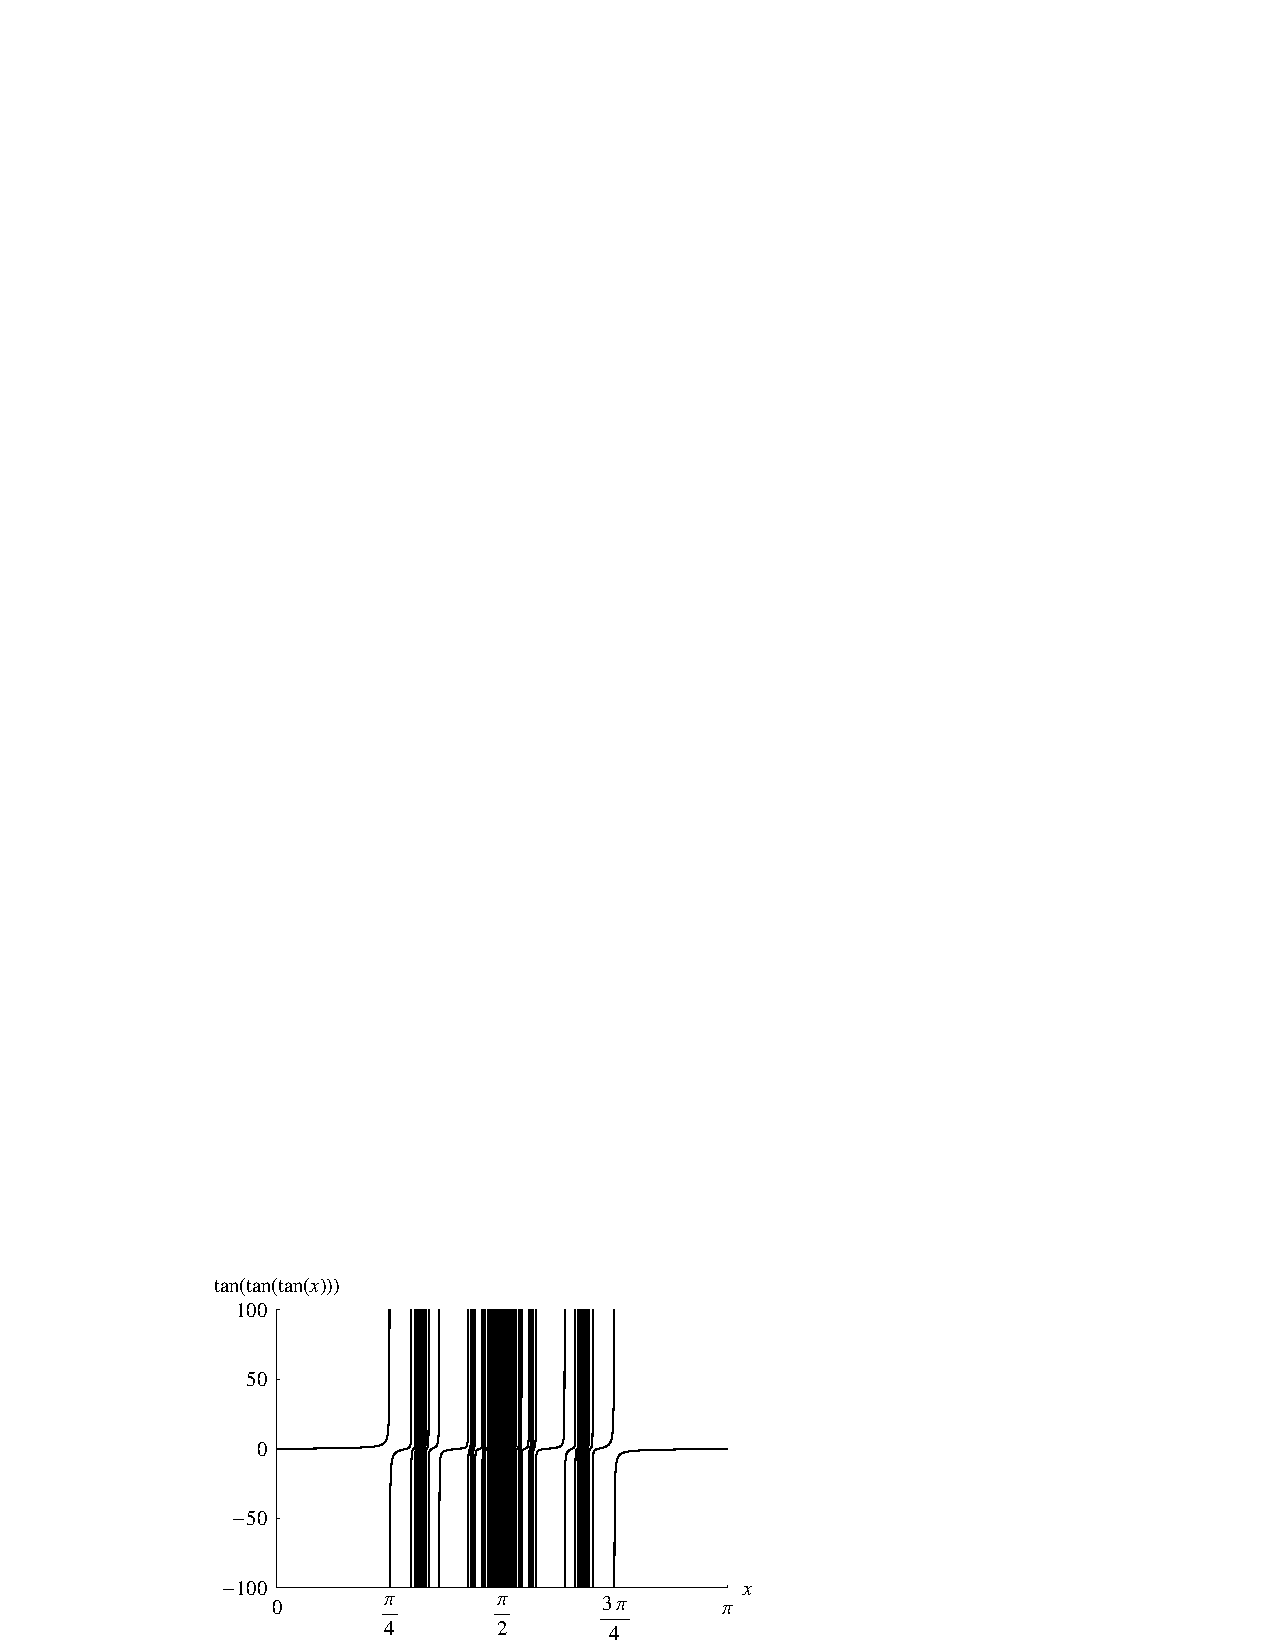
\includegraphics[scale=0.668]{tan3.pdf}
\end{center}
\caption{Graph of  $\tan^{[2]}(x)$ (left) and $\tan^{[3]}(x)$ (right).}
\end{figure}

This paper is a brief companion for the original paper by Bornemann and Schmelzer. The approach taken here could probably be extended for a larger class of functions. This would require a careful analysis shading light away from the central ideas. 
However, Bornemann and Schmelzer \cite{BornemannSchmelzer} gave already an elementary proof for a large class of functions and therefore our focus is on a short and elegant analysis using tools from Fourier analysis.

\section{Into Fourier space and back again}
The Fourier transform of $f$ exists but does not have to be integrable. This is an additional requirement for the analysis given here.
If both $f$ and its Fourier transform
\[
\hat{f}(\xi) := \int_{-\infty}^{\infty} f(x)\ e^{- 2\pi i x \xi}\,dx,\qquad \xi \in \R
\]
are integrable then for almost every $x$ (and for all $x$ if $f$ is continuous) 
$f$ can be represented as the inverse transform of $\hat f$
\[
f(x) = \int_{-\infty}^\infty \hat f(\xi) e^{2 i \pi x \xi} \, d\xi.
\]
And therefore
\[
f(\tan^{[n]}x) = \int_{-\infty}^\infty \hat f(\xi) e^{2 i \pi \xi \tan^{[n]}x} \, d\xi.
\]
We insert the this term into (\ref{eq1}) and restate the problem as
\[
I_n[f] = \frac{1}{\pi}\int_0^\pi \int_{-\infty}^\infty \hat f(\xi) e^{2 i \pi \xi \tan^{[n]}x} \, d\xi \,dx.
\]
Since $\hat f$ is integrable the integral
\[
\frac{1}{\pi}\int_0^\pi \int_{-\infty}^\infty \abs{\hat f(\xi) e^{2 i \pi \xi \tan^{[n]}x}} \, d\xi \,dx
\]
exists. We can therefore apply Fubini's theorem and get
\begin{equation}\label{eq3}
I_n[f] = \int_{-\infty}^\infty \hat f(\xi) \frac{1}{\pi} \int_0^\pi  e^{2 i \pi \xi \tan^{[n]}x} \,dx \,d\xi. 
\end{equation}
\section{The inner Fourier integral}
Still the problem does not look any simpler. The Hydra is lurking now in the inner integral
\begin{equation}\label{Fourier1}
\frac{1}{\pi} \int_0^\pi  e^{2 i \pi \xi \tan^{[n]}x} \,dx \qquad \xi \in \R.
\end{equation}
The $\tan$ function maps the upper halfplane into itself.
Therefore for $\xi \geq 0$ the integrand is bounded in the upper halfplane. We get using dominated convergence
\[
\lim_{\epsilon\downarrow 0} \frac{1}{\pi} \int_0^\pi  e^{2 i \pi \xi \tan^{[n]}(x+\epsilon\,i)} \,dx =  \frac{1}{\pi} \int_0^\pi  e^{2 i \pi \xi \tan^{[n]}x} \,dx \qquad \xi \geq 0.
\]
The function  $e^{2 i \pi \xi \tan^{[n]}z}$ is analytic in the upper halfplane and therefore we can apply Cauchy's theorem.
As a contour we choose the rectangle with corners $(0,\epsilon\,i),(\pi,\epsilon\,i),(\pi,a\,i),(0,a\,i)$. 
The contributions from both vertical vertexes vanish as $\tan$ is periodic. And therefore
\[
\lim_{\epsilon\downarrow 0}  \frac{1}{\pi} \int_0^\pi  e^{2 i \pi \xi \tan^{[n]}(x+\epsilon\,i)} \,dx = \frac{1}{\pi} \int_0^\pi  e^{2 i \pi \xi \tan^{[n]}(x+a\,i)} \,dx \qquad \xi \geq 0, a > 0.
\]
Hence we can integrate on any parallel line above the real line. In the extreme case we can move $a$ towards infinity and as
\[
\lim_{a \uparrow \infty} \tan^{[n]}(x+a\,i)= i \tanh^{[n-1]}1
\]
we get
\[
\frac{1}{\pi} \int_0^\pi  e^{2 i \pi \tan^{[n]}x \xi} \,dx = e^{-2 \pi \xi \tanh^{[n-1]}1} \qquad \xi \geq 0.
\]
For $\xi \leq 0$ the same argument applied in the lower halfplane yields
\[
\frac{1}{\pi} \int_0^\pi  e^{2 i \pi \tan^{[n]}x \xi} \,dx = e^{2 \pi \xi \tanh^{[n-1]}1} \qquad \xi \leq 0.
\]
For $n \to \infty$ both integrals converge to $1$ and hence
\[
\lim_{n \uparrow \infty} I_n[f] = \int_{-\infty}^\infty \hat f(\xi)\,d\xi = f(0).
\]  
In the last step we have applied Parseval's theorem.

\section{From Fourier to Hardy}
Comparing Equation (\ref{Fourier1}) and Equation (\ref{eq1}) reveals that the inner Fourier integral is just a special case of (\ref{eq1}) with $f(x) = e^{2 i \pi \xi x}$.
It may seem that we have made use of special properties of this particular function $f(x)$, but in fact the results generalises for a larger class of functions $f$.
To transfer our arguments from above we need to assume that $f(z)$ is analytic and bounded in the upper halfplane. 
However, the space of bounded analytic functions in the upper halfplane is the Hardy space $H^{\infty}$. 
So, let $F \in H^\infty$, then $\|F\|_{H^\infty} = \sup_{\Im z > 0}|F(z)| < \infty$. The function $f$ may be interpreted as the non-tangential limit of $F$, that is $f(x) = F(x+iy)$ for $y \downarrow 0$. This implies $f$ is bounded, too.


Assuming that $f$ is continuous and bounded on the real line this resembles a kind of boundary value problem. However, the analytic extension of $f$ is rarely bounded in the upper halfplane.

Now, from potential theory (see \cite[Thms. 15.1a, 15.4d]{Hen}) we know that there is a function $F(z)$, holomorphic
in the upper complex half plane $\Im z >0$, such that the harmonic function $\Re F(z)$ is bounded and has boundary values given by $f$, that is,
\begin{equation}\label{eq.F}
\Re F(x+ i y) \to f(x), \qquad x\in\R,
\end{equation}
as the real number $y$ approaches zero from above. The holomorphic function $F$ is \emph{unique}
up to a purely imaginary additive constant. For the sake of simplicity of our presentation, we will further
{\em assume that $F$ itself, not just $\Re F$, is bounded}\/; this additional assumption will be dropped
in the elementary, real analysis proof of Section~\ref{sect.real}.

Therefore
\[
\frac{1}{\pi}\int_0^\pi f(\tan^{[n]}x)\,dx = \Re \frac{1}{\pi} \int_0^\pi F(\tan^{[n]}x)\,dx = \Re F(i \tanh^{[n-1]}1)
\]

Still the assumptions on $f$ are fairly strong. 

\begin{thebibliography}{9}                                                                                                %
\bibitem {BornemannSchmelzer}\textsc{F. Bornemann and T.Schmelzer}, \textit{Taming a Hydra of Singularities},
American Mathematical Monthly, \textbf{114}(8), (2007), 727-732.
\end{thebibliography}
\end{document}
